\documentclass[tikz,border=8pt]{standalone}
\begin{document}
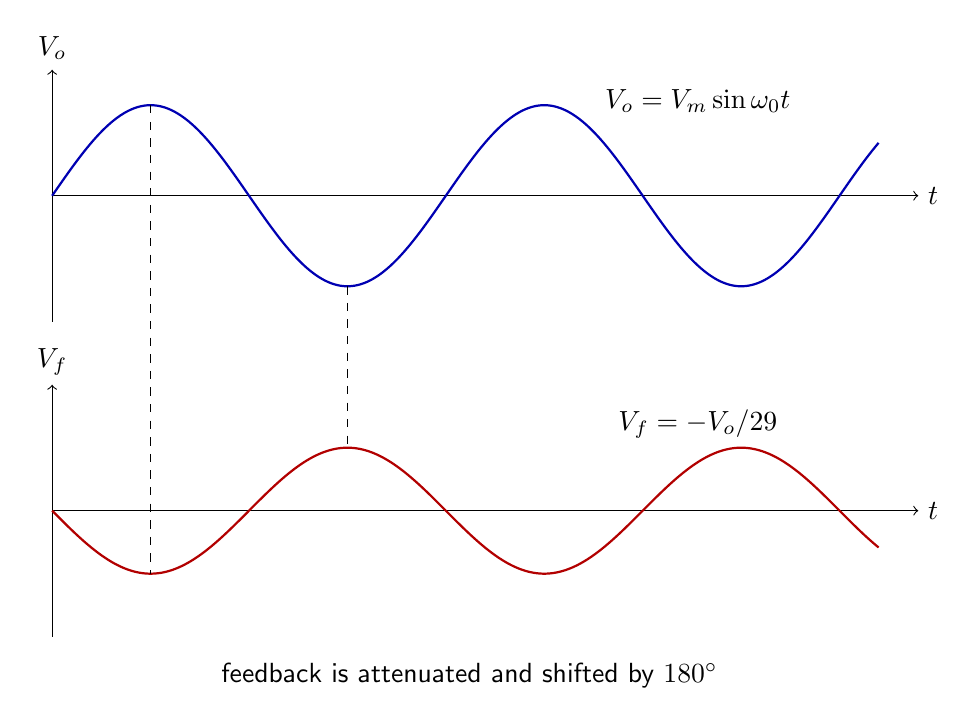
\begin{tikzpicture}[font=\sffamily,x=1cm,y=1cm]
\draw[->] (0,0)--(11,0) node[right]{$t$};
\draw[->] (0,-1.6)--(0,1.6) node[above]{$V_o$};
\draw[blue!70!black,thick,domain=0:10.5,samples=400] plot (\x,{1.15*sin(72*\x)});
\draw[->] (0,-4)--(11,-4) node[right]{$t$};
\draw[->] (0,-5.6)--(0,-2.4) node[above]{$V_f$};
\draw[red!70!black,thick,domain=0:10.5,samples=400] plot (\x,{-4-.8*sin(72*\x)});
\draw[dashed] (1.25,1.15)--(1.25,-4.8);
\draw[dashed] (3.75,-1.15)--(3.75,-3.2);
\node at (8.2,1.2) {$V_o=V_m\sin\omega_0t$};
\node at (8.2,-2.9) {$V_f=-V_o/29$};
\node[align=center] at (5.3,-6.1) {feedback is attenuated and shifted by $180^\circ$};
\end{tikzpicture}
\end{document}
